
\subsection{Extending the Tor protocol}

We extend the Tor routing protocol described in Tor's
specifications~\cite{dingledine2018tor} and we exploit Tor's leaky-pipe circuit
topology\footnote{``Leaky pipe'' refers to the ability of the user to direct
  traffic that ends at an intermediate hop along the circuit} to exchange
payment information with each hop of the circuit. We introduce two new control
cell types: one link-level cell and one relay-level cell. The link-level cell is
used to exchange information related to the payment protocol between the Tor
client and its guard relay while the relay-level cell is used for the middle
relay and the exit relay. This subtype of relay cell is comprised of a payment
header denoting the type of payment cell, followed by a payload of payment
data. To an outside observer, payment cells are indistinguishable to normal
relay cells. Figure~\ref{fig:relay_command_mt_structure} shows the internal structure of the cell.
\begin{figure}[h]
    \centering
    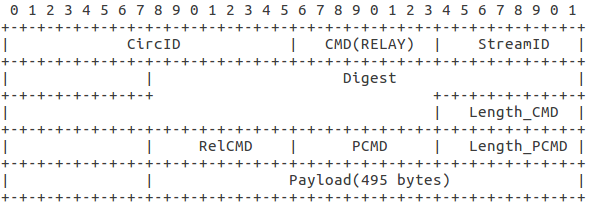
\includegraphics[scale=0.38]{images/payment_cell_header.png}
    \caption{Relay level payment cell structure}
\label{fig:relay_command_mt_structure}
\end{figure}

All the bytes starting from StreamID (included) are onion-encrypted. RelCMD is set to RELAY\_COMMAND\_MT, PCMD is the payment command which is different for each step of the payment protocol. If some message overflow the payload available length (495 bytes), we queue multiple cells of the same PCMD and buffer them on the receiver side to unpack the whole message.

\subsection{Channels are pre-built}
Tor already follows the
same strategy with streams: a circuit must be ready before a stream is created,
such that it can be attached to a ready circuit and sends its data directly
through the anonymous tunnel. Similarly, moneTor allows secure and anonymous
payment channels to be pre-built over an unused clean circuit, which allows the Tor client to hold some payment circuit in reserve. Our implementation features some initial predict and pre-built strategy, where the Tor client is able to predict to some extend the number of pre-build channels to create using previous usage information. However, the approach is somewhat prototyped, and Tor may need cleverer strategy not to exhaust the network's resource by pre-building unnecessary nanopayment channels.

\subsection{Scalability of the moneTor Scheme}
\label{subsub:scalability}
%\td{TODO: describe scalability of intermediary system and any networking
%  bottlenecks that might arise such as port limits, etc.}

In our design, we are concerned with memory consumption, kernel socket
consumption and CPU consumption. Our choice for a tripartite protocol
effectively shifts the memory consumption of opened and idle micro channels to
the Intermediary nodes of the network. A more basic setup whereby each Tor
client maintains a micropayment channel with each relay would incur an $O(n*m)$
cost with respect to channel management complexity. By engineering an additional
intermediary layer, the complexity of moneTor channel connections is reduced to
$O(n+m)$. In our implementation, Intermediary relays do not participate in
routing user streams and are tasked only with providing payment channel
services. Intermediaries devote the full extent of their computational resources
toward this task allowing only a few strong nodes to handle all of the premium
channel establishments required the network.

%\td{Should we emphaisize more the need to anonymousely manage circuits between
%  parties? Or is this obvious?}
%FR: looks obvious to me from the phrase below
Interactions between parties are realised within Tor circuits to allow
multiplexing of circuits over the same TCP connection. As a result, the
intermediary and the ledger must have a number of available sockets higher than
the number of relays in the network in the worst case. Since this limit is in
line with Tor's current assumption, our design inherits the same socket
consumption scalability of the greater Tor network.

\subsection{Prioritized Traffic}
\label{subsub:prioritized}

The final component of our network-oriented design addresses the need to deliver
prioritized bandwidth given an explicit signaling of premium or nonpremium
traffic. Our objective is to provide a tunable range of prioritization while
incurring as little cost as possible to average global performance. Traffic
scheduling is perhaps the most intuitive mechanism with which to implement
priortization. However, we found in our investigation that practical
modification of the Tor scheduling infrastructure is nontrivial. A more detailed
discussion of our findings can be found in Appendix~\ref{sec:scheduling}.

Fortunately, Tor's overlay flow control mechanism provides an alternative route
to implement our desired functionality. Recall that edge nodes regulate the
traffic flux in either direction using a set of flow control windows. Roughly
speaking, these windows determine space allotted to each circuit on a relay's
scheduling queue, which in turn is positively correlated with effective
bandwidth. AlSabah \textit{et al.}~\cite{pets2011-defenestrator} have explored
the affects of changing flow control windows as a way to improve total
performance. Our objective slightly differs: we want to improve the performance
of a subset of premium users, at the cost of decreasing the performance for
unpaid bandwidth.  We implement our prioritization scheme by readjusting the
windows according to the following formula.
\begin{equation}
  window' = window(1+ \alpha(premium / premium\% - 1))
  \label{eq:flow}
\end{equation}
Here, a circuit is marked as prioritized by the bit $premium \in \{0, 1\}$. The
tunable priority benefit $\alpha \in [0, 1)$ defines the total amount of flow
capacity we wish to transfer to premium clients. Accounting for
$premium\%s \in [0,100]$, the fraction of premium to nonpremium clients, we can
keep the total flow capacity constant. Our policy may be implemented in one of
two ways. First, each node could track the $premium\%$ locally and dynamically
adjust their own windows. This introduces a considerable amount of added
complexity with unclear consequences on network performance. A more sound
approach calls for the Tor authorities to track the global value for $premium\%$
and periodically broadcast static flow control windows to be used by the entire
network. We adopt the latter approach in this iteration of moneTor.
%\footnote{Our
%  research in traffic prioritization is meant to demonstrate at least some crude
%  capacity for premium advantage in our models and to suggest potential avenues
%  for further study. A more definitive design for production-ready policies is
%  left for future networking-oriented research.}
